\documentclass[border=10pt]{standalone}
\usepackage{tikz}\usepackage{amsmath}\usetikzlibrary{arrows.meta,calc}
\begin{document}
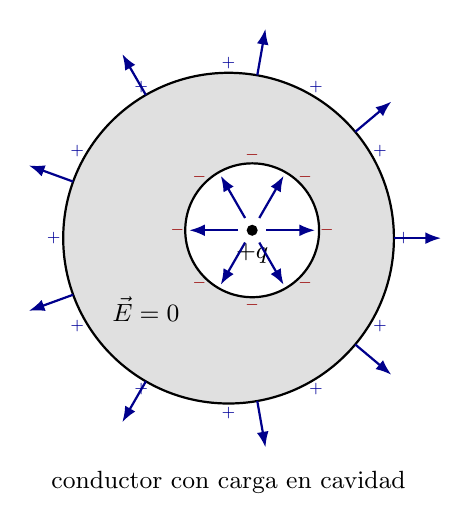
\begin{tikzpicture}[line width=0.8pt,>={Latex[length=2mm]}]
  \draw[thick,fill=black!12] (0,0) circle(2.1);
  \draw[thick,fill=white] (0.3,0.1) circle(0.85);
  \fill (0.3,0.1) circle(2pt) node[below=1pt]{\small$+q$};
  % campo en cavidad
  \foreach \a in {0,60,...,300} \draw[->,blue!55!black] ($(0.3,0.1)+(\a:0.18)$)--($(0.3,0.1)+(\a:0.8)$);
  % carga inducida pared cavidad (-) y exterior (+)
  \foreach \a in {0,45,...,315} \node[red!60!black] at ($(0.3,0.1)+(\a:0.95)$){\tiny$-$};
  \foreach \a in {0,30,...,330} \node[blue!60!black] at (\a:2.22){\tiny$+$};
  \node at (-1.05,-0.9){\small $\vec E=0$};
  % campo exterior radial
  \foreach \a in {0,40,...,320} \draw[->,blue!55!black] (\a:2.1)--(\a:2.7);
  \node at (0,-3.1){\small conductor con carga en cavidad};
\end{tikzpicture}
\end{document}
